\section{Testing eBPF programs}\label{sec:testing}
The compiler integrates an end-to-end testing framework to verify the 
correctness of a P4-eBPF/XDP program. The framework consists of a user space 
and a kernel testing pipeline. Both run a test from the compilation 
till the actual runtime deployment of a P4 program.

\subsection{Why Test in User-Space?}
Testing in user space isolates the specification of the eBPF program from the
implementation. It is primarily intended to test the correctness of the
compiler and the generated C code without interference of the kernel verifier
and tooling. The user space testing framework does not depend on the LLVM
compiler or specific kernel version. It also does not require usage of iproute2 
tooling such as tc or ip. Our aim is to ensure that a P4 program is functionally
equivalent to its corresponding XDP C-code.

Testing in user space also ensures debugging simplicity for the average
user. Tools such as GDB, valgrind, wireshark, or simple output statements
are readily available.

\subsection{The Simple Test Framework}
\begin{figure}
	\centering
	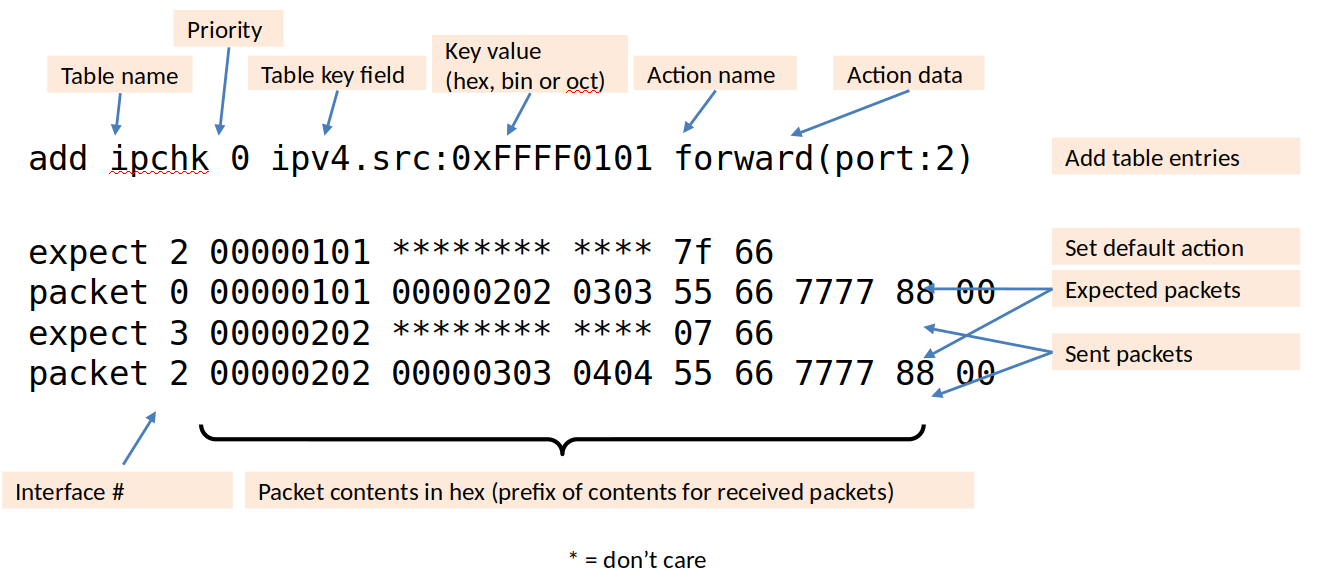
\includegraphics[width=\linewidth]{stf}
	\caption{Simple testing framework program fragment for exercising P4 programs.}
	\label{fig:stf}
\end{figure}
The simple test framework (STF) is a dataplane verification language. 
An STF template defines a set of actions which are sequentially executed on the 
dataplane.

An example STF action is \texttt{packet}. \texttt{packet} describes the 
byte content of an inbound Ethernet frame and the port which will receive the 
packet.
Its counterpart, \texttt{expect}, defines which port will send out an Ethernet 
frame. This implies we \textit{expect} our dataplane to forward the frame 
given by \texttt{packet} to the port in the command.
The action \texttt{add} on the other hand is a simple PUT operation on 
dataplane tables. It describes which table to update and what key-value pair to 
insert.

While its original purpose is to assess switching and forwarding behavior, STF 
templates can also be used to test eBPF programs in isolation. The P4 compiler 
features a parser, which pre-processes the templates and generates an ordered 
command list. This list is interpreted by the eBPF testing framework, 
which produces pcap files from the \texttt{packet} commands and converts 
\texttt{add} operations into eBPF map syscalls.
Table \ref{table:stf} describes the full list of commands that are currently 
supported.

\paragraph{Example}
An example of an STF template can be seen in Figure \ref{fig:stf}. \texttt{add} 
defines that, if the IPv4 source address of a packet matches with the key in 
table \texttt{ipchk}, we forward the packet to 
port 2. After the table update, the template specifies to insert packets on 
port 0 and 2 and to expect output packets on port 2 and 3.


\begin{table*}[h]
	\begin{center}
		\begin{tabular}{|l|p{9cm}|} \hline
			\textbf{Command} & \textbf{Description} \\ \hline \hline
			\textbf{packet} port data & Insert a frame of bytes
			\textit{data} into port \textit{port}.    \\ \hline
			\textbf{expect} port data & Expect a frame of bytes
			\textit{data} on port \textit{port}.  \\ \hline
			\textbf{add} tbl priority match action & Insert a
			match-action entry with key \textit{match} and action
			\textit{action} into table \textit{tbl}. \\ \hline
			\textbf{setdefault} tbl action & Set the default action for table
			\textit{tbl}. \\
			\hline
			\textbf{check\_counter} tbl\_name key == n & Check if the value on
			the entry \textit{key} in counter table \textit{tbl} matches
			\textit{n}.  \\
			\hline
			\textbf{wait} & Pause any operation for a second. \\ \hline
		\end{tabular}
		\caption{The STF command palette.}\label{table:stf}
	\end{center}
\end{table*}

\subsection{The Test Runtime}
A P4C-XDP test is an end-to-end verification of all stages of 
the compilation pipeline. This includes verifying that the P4 code does 
compile, that the generated eBPF/XDP C is correct, and that the actual runtime 
behavior of the loaded program matches expectations.

\subsubsection{Architecture}
The test infrastructure is designed to be flexible and independent of the 
target backend. New testing frameworks can be added by creating a target file 
and linking it to the P4C test target folder. Each test will pass through five 
abstract test stages:\\

\noindent\textbf{compile-p4}\\ Compile the P4 file to a dataplane binary. \\
\textbf{parse-stf}\\ Parse the stf file and interpret the output. \\
\textbf{compile-dataplane}\\ Load the P4 binary and create a runtime.\\
\textbf{run}\\ Start the runtime and read in the STF file inputs.\\
\textbf{check-results}\\ Compare the results with the STF 
expectations.\\

The implementation of these stages is up to the compiler backend.
Currently, both eBPF/XDP kernel and user space targets are supported.

The user space testing framework defines a set of eBPF wrappers to approximate 
the kernel implementation. eBPF maps are implemented as simple hash maps, the 
map file descriptor API is emulated by a common registry. Functionality is 
limited and only extends to the minimal eBPF map operations necessary for 
filtering and classifying.

Every target in the eBPF compiler is required to implement a custom 
\textit{target header}. This target header specifies how macros in the eBPF 
source file are expanded. For example, \texttt{ebpf\_test.h} defines 
\texttt{BPF\_MAP\_LOOKUP\_ELEM} to call into the userspace registry whereas 
\texttt{ebpf\_kernel.h} defines the function as the standard eBPF system call.

\subsubsection{Running a Test}
A test requires only an STF template and a P4 program as input. The 
remaining files are generated or linked. The five testing stages are 
implemented as follows:\\

\noindent\textbf{compile-p4}\\
Depending on the backend the P4 program is either compiled to eBPF or 
to XDP C-Code. A header file accompanies the generated program. This stage 
verifies that the P4 program matches the expected syntax.\\ 
\textbf{parse-stf}\\
The framework parses the associated STF file and generates a set of input pcap 
files per port. The expected output packets are stored in a map for later use. 
In addition, all \texttt{add} operations are converted to eBPF map calls and 
exported as control file.\\
\textbf{compile-dataplane}\\
Once the P4 and STF file have been parsed, the framework compiles 
the eBPF C program, the eBPF wrappers, and the control plane operations into a 
test runtime.

This runtime initializes all eBPF tables with entries specified by the STF 
file, then "runs" the dataplane by processing a set of input packets.
As input the runtime takes a set of pcap files, which are spliced into per-port 
lists and individually inserted into the datapath.
As the pcapng format, which contains port information as packet metadata, is 
not yet supported by libpcap, we identify the input port of a pcap file by
its filename.

In addition to creating the runtime, the kernel version compiles the eBPF/XDP 
program to an eBPF object using clang and llvm.\\
\textbf{run}\\
At this point, the user and kernel frameworks diverge in behavior.

In the user space version, packets are converted to a mock-sk\_buff structure 
and then directly passed into the to-be-tested eBPF/XDP function call. The 
output result is recorded and written to per-port output pcap files.

The kernel framework, however, is intended to verify the correctness of an 
eBPF/XDP object in relation to the host kernel. This results in a more complex 
pipeline (See Figure \ref{fig:kernel_test}). 
Before the eBPF program is loaded, the framework creates a bridge running in an 
network namespace. Isolation via a namespace ensures that existing 
virtual interfaces and eBPF maps do not conflict with the test in question.
\texttt{n} virtual interfaces are attached to the bridge, corresponding to 
the highest port identifier defined in the STF file.

The compiled eBPF object is then loaded into all ports using \texttt{tc} or 
\texttt{ip}. Instead of directly calling into the eBPF program, the kernel 
runtime writes the packet to the associated port using raw sockets. The output 
results are recorded by sniffing on the interfaces via tcpdump.\\
\textbf{check-results}\\
After the program has completed, the results are collected and compared with 
the expected packets defined by the STF template. If the output port or the 
dataframe content does not match the specification, the test returns an error 
code and is marked as failed.

Both the user and kernel space runtime do not support testing for counters 
and table state yet. We have planned these extensions as future work.
\begin{figure}
	\centering
	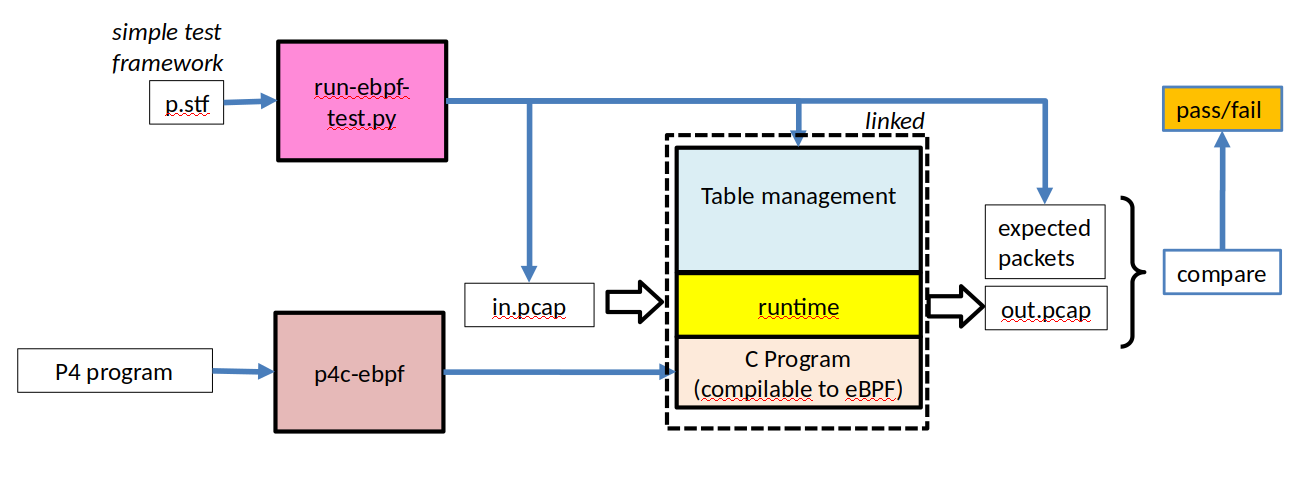
\includegraphics[width=\linewidth]{user_test}
	\caption{User-level testing of the C programs generated by the P4 compilers.}
	\label{fig:user_test}
\end{figure}
\begin{figure}
	\centering
	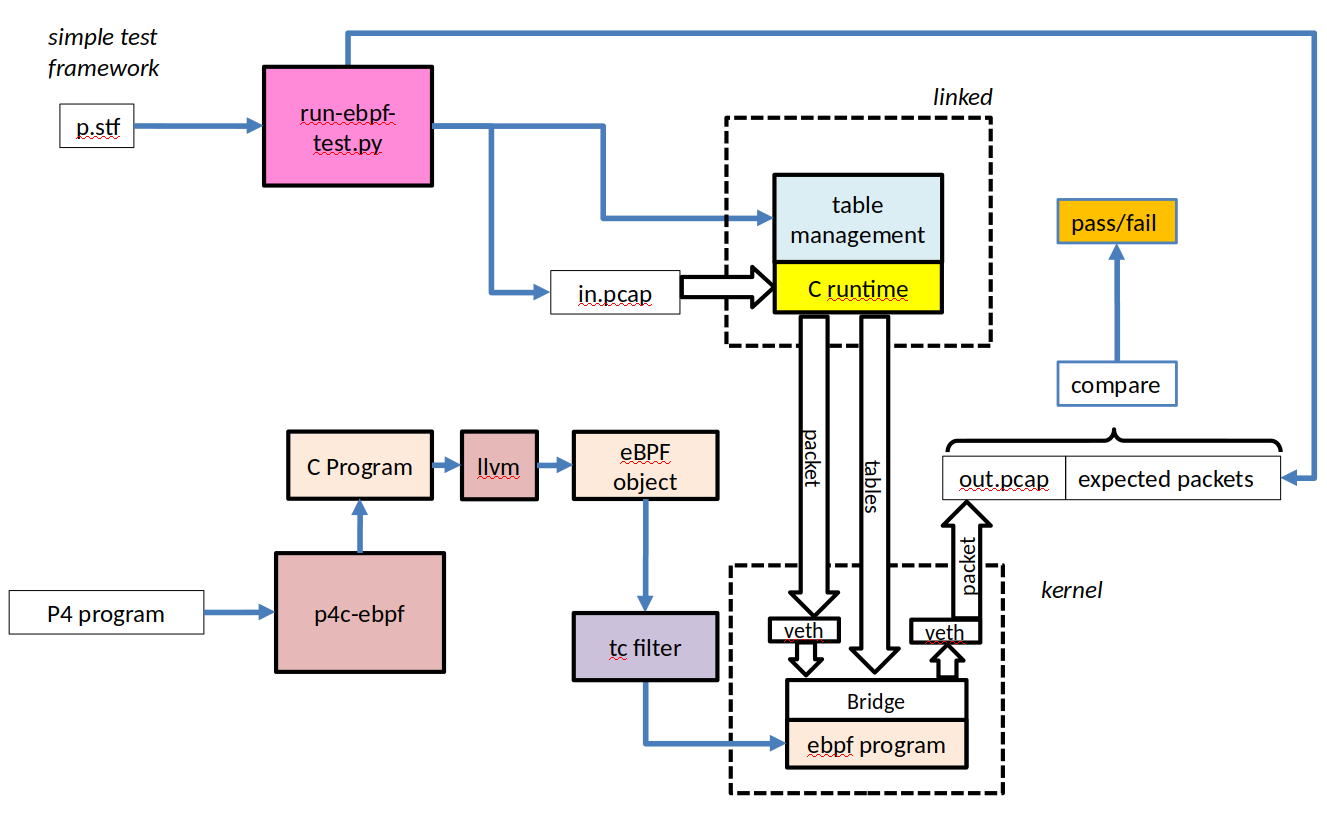
\includegraphics[width=\linewidth]{kernel_test}
	\caption{Kernel-level testing of the C programs generated by the P4 
	compilers.}
	\label{fig:kernel_test}
\end{figure}
\subsubsection{Using the Test Runtime}
The test framework can be used independently to verify eBPF and XDP programs. 
[TODO] Talk about how you test raw ebpf C programs with having a P4 template. 
The idea is that we can use the backend to also just test random eBPF/XDP 
programs with our compiler. I have not been able to implement this yet.
Also talk how to use:
\begin{lstlisting}[language=bash]
make -f p4c/backends/ebpf/runtime/kernel.mk \
	BPFOBJ=out.o P4FILE=PROGRAM.p4
\end{lstlisting}
to directly compile P4 to an eBPF object.
